\chapter{Background}
To deliver an all round level of comprehension the following section discusses generic terms which are used throughout the project such as Big Data (Section \ref{bigdata}) and Extract Transform Load (Section \ref{etl})

\section{Big Data}\label{bigdata}
Big Data is a broad evolving term bound to a complex and powerful application of analytical insight which over recent years has had a variety of definitions. In simplistic terms Big Data can be described as extremely large datasets that may be studied computationally to reveal patterns, trends, and associations for ongoing discovery and analysis.

\subsection{3vs Model}
In 2001, Gartner analyst Doug Laney delivered the original 3vs model which categorises big data in to three dimensions; Volume, Variety and Velocity.  The characteristics of each property are defined as \textbf{Volume} - The size of the generated data is required to assess whether the dataset is in fact 'big' enough to be categorised as Big Data. \begin{wrapfigure}{l}{0.3\textwidth}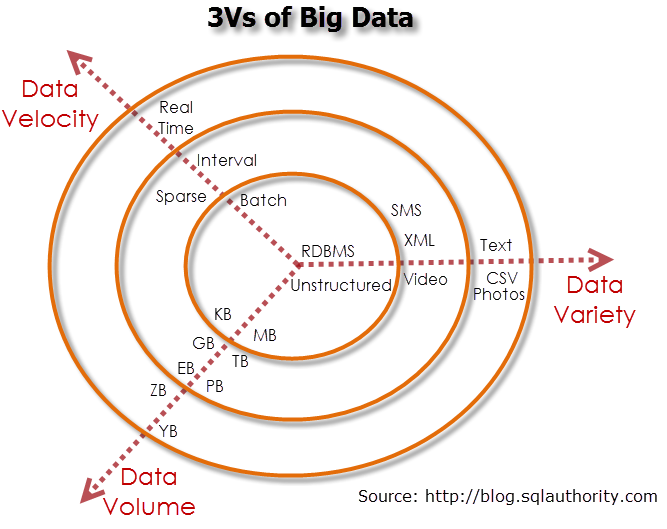
\includegraphics[width = 1\linewidth]{images/3vs}\end{wrapfigure} \textbf{Variety} - The type of content, and an essential fact that data analysts must know. This helps people who are associated with and analyze the data to effectively use the data to their advantage and thus uphold its importance.\textbf{Velocity} - In this context, the speed at which the data is generated and processed to meet the demands and the challenges that lie in the path of growth and development. \textbf{Variability} - The inconsistency the data can show at times?-which can hamper the process of handling and managing the data effectively. \textbf{Veracity} - The quality of captured data, which can vary greatly. Accurate analysis depends on the veracity of source data. Laney's 2001 publication \textit{3D data management: Controlling data volume, variety and velocity} is still widely recognised today as the expansion of all three properties encapsulate the challenges currently faced of big data management.

\section{Extract Transform Load}\label{etl}
A basic definition of the Extract Transform Load (ETL) process is pulling data out of one database, refactoring the composition of the data and putting the data into another database. 

\subsection{Process}
ETL is a three step procedure which combines database functions into one tool.
\subsubsection{Extract} is the first step in the ETL procedure in which data is read from a database. The Extract step covers the data extraction from the source system and makes it accessible for further processing. The main objective of the extract step is to retrieve all the required data from the source system with as little resources as possible. The extract step should be designed in a way that it does not negatively affect the source system in terms or performance, response time or any kind of locking.
\subsubsection{Transform} where the extracted data is manipulated from its previous state and converted into another database format. The transform step applies a set of rules to transform the data from the source to the target. This includes converting any measured data to the same dimension (i.e. conformed dimension) using the same units so that they can later be joined. The transformation step also requires joining data from several sources, generating aggregates, generating surrogate keys, sorting, deriving new calculated values, and applying advanced validation rules.
\subsubsection{Load} completes the three step procedure and is where data is written into the target database. During the load step, it is necessary to ensure that the load is performed correctly and with as little resources as possible. The target of the Load process is often a database. In order to make the load process efficient, it is helpful to disable any constraints and indexes before the load and enable them back only after the load completes. The referential integrity needs to be maintained by ETL tool to ensure consistency.
\subsection{Tool Implementation}
https://jena.apache.org/
There are many ready-to-use ETL tools on the market. The main benefit of using off-the-shelf ETL tools is the fact that they are optimized for the ETL process by providing connectors to common data sources like databases, flat files, mainframe systems, xml, etc. They provide a means to implement data transformations easily and consistently across various data sources. This includes filtering, reformatting, sorting, joining, merging, aggregation and other operations ready to use. The tools also support transformation scheduling, version control, monitoring and unified metadata management. 